\documentclass[11pt]{article}
\usepackage[utf8]{inputenc}
\usepackage[english, ngerman]{babel}
\usepackage{amsmath,amsthm,verbatim,amssymb,amsfonts,amscd}
\usepackage{enumerate}
\usepackage{listings}
\usepackage{courier}
\usepackage{graphicx}
\usepackage[margin=1in]{geometry}
\usepackage{epstopdf}
\lstset{
  numbers=left,
  language=C,
  basicstyle=\footnotesize\ttfamily,
  breaklines=true,
  morekeywords={function, NIL}
}
\newcommand{\abs}[1]{\left| #1 \right| }
\setlength{\parindent}{0pt} 

\author{
  Felix Schrader, 3053850 \\ 
  Jens Duffert, 2843110 \\
  Eduard Sauter, 3053470
}
\title{Datenstrukturen und Algorithmen: Haus\"ubung 4}
\begin{document}
\maketitle

\subsection*{Aufgabe 3}
\begin{enumerate}[a)]
  \item 
    \begin{figure}[h!]
      \centering
      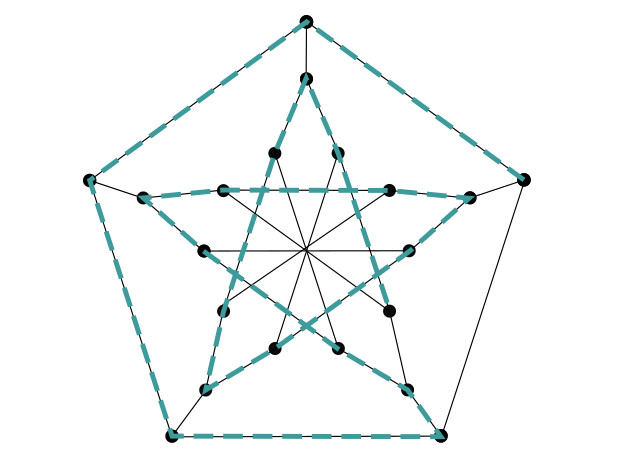
\includegraphics[width=0.8\textwidth]{hamilton_graph}
      \caption{Hamiltonischer Pfad}
      \label{fig:hamilton_graph.eps}
    \end{figure}
  \item
    Es sei $G$ ein Graph $(V, E)$ mit $\abs{V} = n>3$ Knoten.
    %
    \begin{align*}
      |E| =\frac{n^2 - 3n}{2} + 3 = 3-2n \sum_{i=1}^{n} i
    \end{align*}
    %
    
\end{enumerate} 


\end{document}
